%This is the first chapter of the dissertation

%The following command starts your chapter. If you want different titles used in your ToC and at the top of
%the page throughout the chapter, you can specify those values here. Since Columbia doesn't want extra
%information in the headers and footers, the "Top of Page Title" value won't actually appear.

%By using the asterisk to start a new section, I keep the section from appearing in the table of contents.
%If you want your sections to be numbered and to appear in the table of contents, remove the asterisk.



\pagestyle{cu}
\graphicspath{{./Chapter1/Figures/}}
\chapter[Dark Matter][Dark Matter]{Dark Matter}
\label{chap:dark_matter}

For much of the last century evidence of two non-luminous components of our universe has been developing

For much of the last century evidence has been building for two non-luminous components of our universe that are not yet understood.
Dark Energy has been derived to explain the accelerating expansion of the universe and is predicted to compose $\sim70$\% of
matter throughout the universe.  Dark Matter is used to satisfy the need for an additional massive component and is expected to
constitute $\sim26$ \% of the universe.  The term "dark" is a relic from their early history and today both are understood to be
invisible.



%====================================
\section[$\Lambda$ CDM Model][$\Lambda$ CDM Model]{$\boldsymbol{\Lambda}$CDM Model}
The cosmological model describes the evolution of the universe since its inception of the Big Bang.  It validity is dependent
on the premise that our universe is homogeneous and isotropic over large ($\sim 100 Mpc$) - consistent with observations,
Einstein's General Relativity, and a path connected universe.  This can be solved for the Robertson-Walker metric, which in
polar coordinates gives

\begin{equation}
ds^{2} = -c^{2}dt^{2} + a(t)^{2} \bigg( \frac{dr^{2}}{1 - kr^{2}} + r^{2}d\Omega^{2} \bigg)
\end{equation}

\noindent where ds is the distance traversed in space-time, $a(t)$ is the scale factor ($a=1$ today), and $k$ is the curvature of the
universe and can be -1, 0, or 1 for open, flat, or closed, respectively.  These values are also known as hyper-spherical,
Euclidean, or spherical.

Solving Einstein's equations with this metric gives the Friedman Equations

\begin{equation}
\Big(\frac{\dot{a}}{a}^{2}\Big) = \frac{8\pi G \rho}{3} - \frac{k}{a^{2}}
\label{eq:friedman1}
\end{equation}

\begin{equation}
\Big(\frac{\ddot{a}}{a}\Big) = -\frac{4\pi G \rho}{3}(\rho + 3p)
\label{eq:friedman2}
\end{equation}

\noindent where $\rho$ is the average energy density of the universe, $\frac{\dot{a}}{a}$ is defined as the Hubble
constant H ($H_{0}$ today), and $p$ is the pressure from components.  From \eqref{eq:friedman1} the critical
density, defined as the density for a flat universe, is $\rho_{crit} = \frac{3H^{2}}{8\pi G}$.  A useful
notation then is the ratio of the density to the critical density, $\Omega = \frac{rho}{rho_crit}$
$\Omega = 1$ is a flat universe.  Substituting
$\Omega$ into \eqref{eq:friedman1} gives the density parameter

\begin{equation}
\Omega - 1 = \frac{k}{H^{2}{a^{2}}}
\end{equation}

\noindent  $\Omega = \sum \Omega_{i}$ where $\Omega_{i}$ is a component of the universe.  Current measurements give density
parameters of $\Omega_{b} ~ 0.05$ for baryonic matter, $\Omega_{dm} = 0.26$ for non-baryonic matter, $\Omega_{r} \sim 0$
for radiation, and $\Omega_{\Lambda} \sim 0.68$ for dark energy (see \ref{subsec:cmb}).  Because cold dark matter
and dark energy dominate $\Omega$ this is referred to as the $\Lambda CDM$ model.



%====================================
\section[Evidence for Dark Matter][Evidence for Dark Matter]{Evidence for Dark Matter}
%========
\subsection{Dynamical Contraints} \label{subsec:dynamics}
The first evidence for Dark Matter came in 1933 when Swiss astronomer Fritz Zwicky was observing the Coma Cluster
and noticed the velocity of the galaxies was larger than the total luminous matter.  He argued that if there were
some additional mass that only acted gravitationally this could explain his observations, and estimated this
to be $\sim 400$ times greater than the luminous matter (\citeref{Zwicky1933}).  Today this factor is much
smaller as the observed luminous matter is larger, but the discrepancy persists.  Zwicky coined this
\textit{dunkel Materie} or ``dark matter".  Since then other galaxy clusters have been observed and supported
this claim.

In 1970 Vera Rubin and Kent Ford used $H\alpha$ from H II regions to measure the rotation of stars around the
center of the Andromeda galaxy \citeref{Rubin1970}.  The virial theorem predicts $v(r) = \sqrt{GM(r)/r}$ so
that at large radii the velocity of the galaxies should decrease as $r^{-1/2}$.  Rubin and Ford's observations
contradicted the value $M(r)$ derived from luminous mass.  As with Zwicky's measurement, the results could be
explained by introducing a non-luminous feature - in this case one with $M(r) \sim r$.  Observations of over
one hundred thousand galaxies have since shown similar results, with DM halos containing several times the
luminous mass.

One example is NGC 6501.  The dark halo mass density in \figref{fig:ngc_6501} is estimated as
$\rho (r) = \rho_{0} \Big[ 1 + \Big( \frac{r}{r_{c}} \Big)^{2} \Big]^{-1}$ where $\rho_{0}$ and $r_{c}$
are the central halo mass density and radius, respectively, by fitting a least square to the velocity
distribution \citeref{Begeman1991}.  The left panel shows the mass of luminous matter decreases after
peaking at $\sim2$ kpc, but the DM increases steadily and at $>10$ kpc is proportional to $r$ causing
the rotational velocity to flatten.  Unfortunately, there is no independent model for determining the
masses of a galaxy's disk, bulge, and halo, which makes disassociating the mass of baryonic matter from
DM very difficult.  Most models assume the luminous matter to compose the galaxy's disk and bulge with
the DM constituting its halo \citeref{Sofu2001}.



\begin{figure}[t]
\centering
\captionsetup[subfigure]{labelformat=empty}
\ffigbox[\linewidth]{%
  \begin{subfloatrow}
\ffigbox[\FBwidth][]{\caption{}}{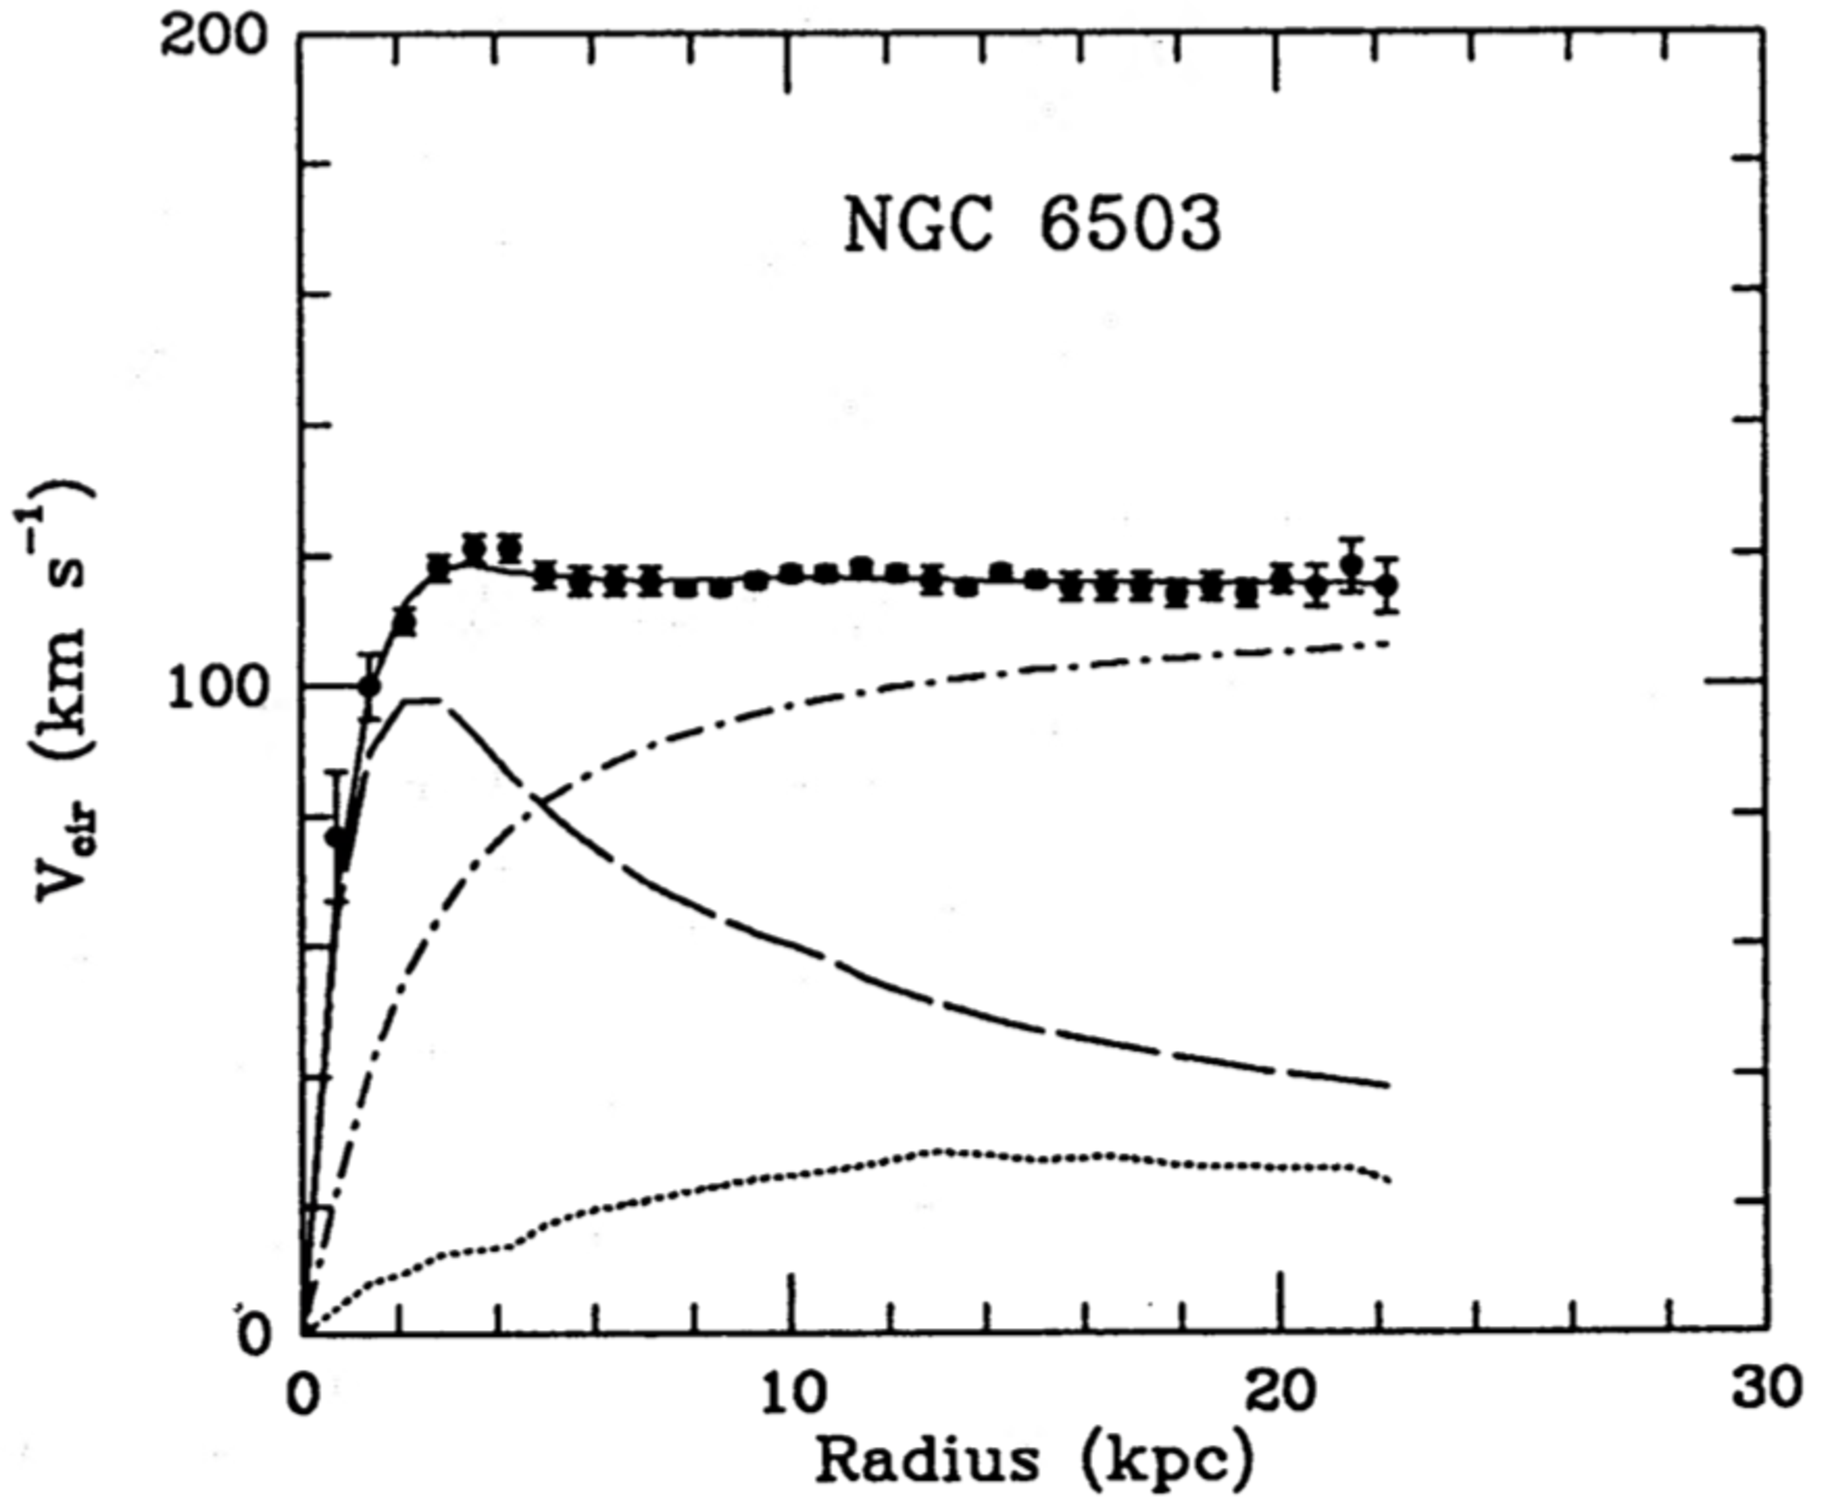
\includegraphics[height=5cm]{ngc_6503}}
  \end{subfloatrow}
  \hspace*{\columnsep}
  \begin{subfloatrow}
\vbox to 5.3cm{
  \ffigbox[\FBwidth]{\caption{}}
  {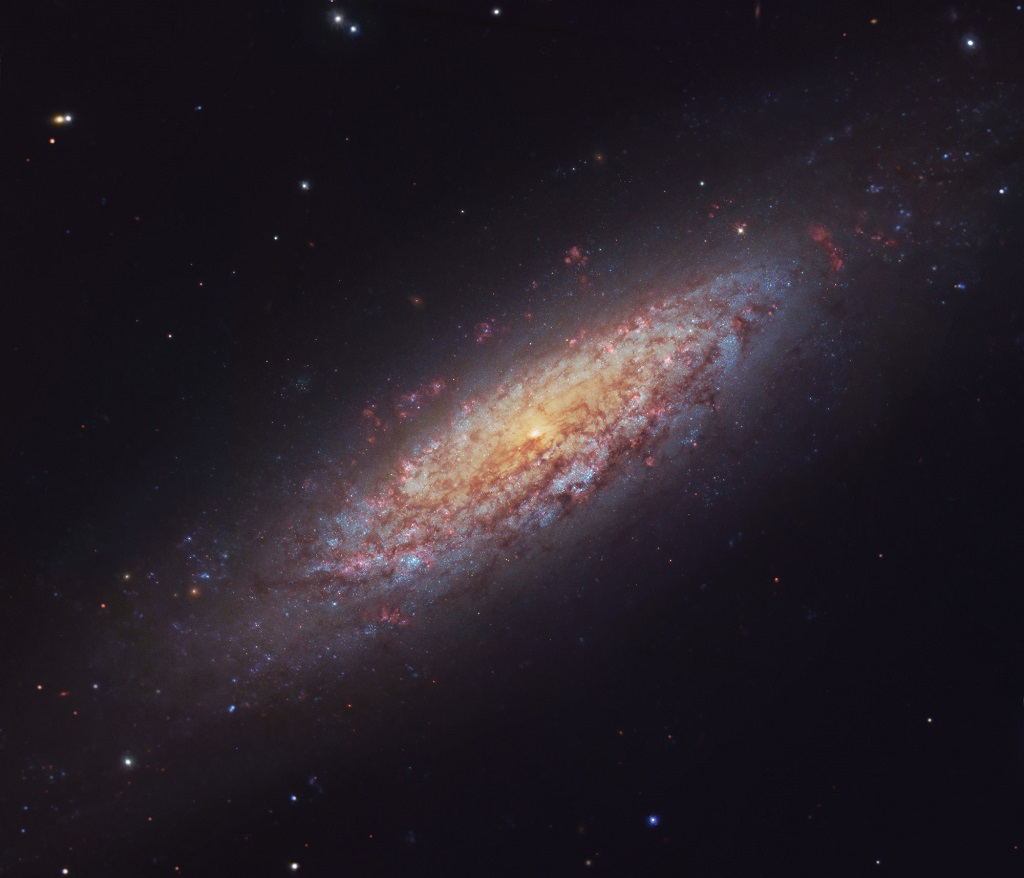
\includegraphics[trim={2cm, 2cm, 2cm, 2cm}, clip, height=4.4cm]{ngc_6503_image}}
}
  \end{subfloatrow}
  }{
  \vspace*{-10mm}
  \caption{(left) Rotational velocity vs. radius for NGC 6503.  Visible components represented by dashed line,
  gas by dotted, and dark halo by dashed-dotted.
Image credit: (left) \citeref{Begeman1991} (right) Robert Gendler, the Subaru Telescope (NAOJ) and the Hubble Legacy Archive}
	\label{fig:ngc_6501}
  }
\end{figure}[t]

%for figure trim info
%https://tex.stackexchange.com/questions/57418/crop-an-inserted-image





\begin{figure}
	\centering
	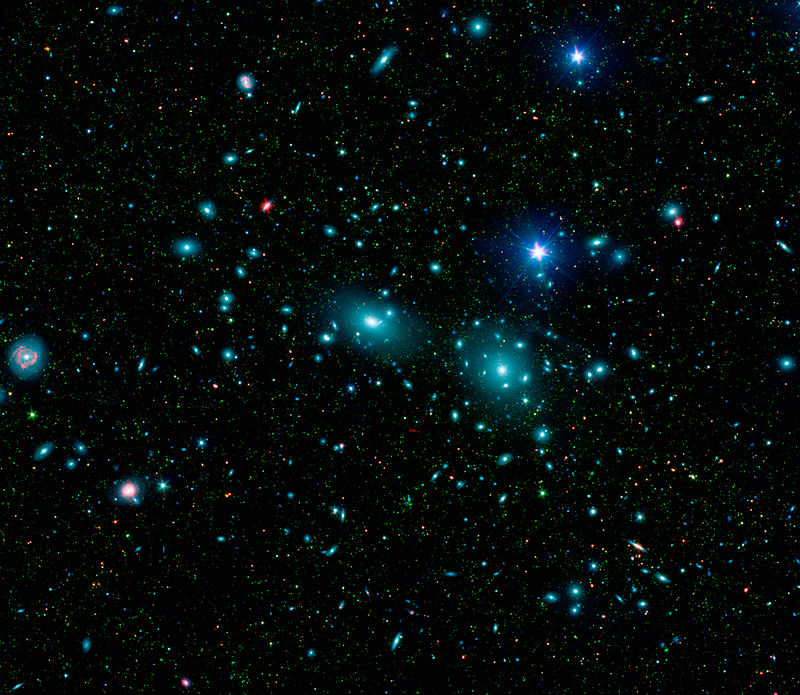
\includegraphics[width=0.5\textwidth]{coma_cluster}
	\label{fig:coma_cluster}
	\caption{Coma Cluster as seen by Sloan Digital Sky Survey and Spitzer Space Telescope.  Image credit: NASA/JPL-Caltech/GSFC/SDSS.}
\end{figure}


%========
\subsection{Big Bang Nucleosynthesis}



%========
\subsection{Gravitational Lensing}
A gravitational lens is a distribution of matter capable of bending electromagnetic radiation between a luminous source and
an observer.  The deflection is caused by the gravitational distortion of space-time by the mass of the lens, which
while in theory can be anything with mass-energy, the effects are typically most noticeable for high-density objects
such as galaxies, galaxy clusters, or a stars.  A source that is gravitationally lensed will have two distinct
features. The convergence, $\kappa$, describes the focusing of the light rays.  The shear, denoted by $\gamma$ and $\phi$, which
represent the ellipticity and position ange, characterizes the distortion of the source.  One important feature of lensing
is a magnification of the source given by

\begin{equation}
\mu = \frac{1}{(1-\kappa)^{2} + \gamma^{2}}
\end{equation}

\noindent that produces an increase in brightness when the source and lens are close to one another.  This has given astronomers
a tool to see objects that previously were thought to be too faint to observe.

In the case of strong lensing an observer will see a misshapen source in the form of arcs.  Because the magnitude of the
deflection is depending on the proximity to the lens, it is possible to see multiple instances of the same source, with
independent distances traveled by each.  Thus a time-delay between images is also present, and their location to the observer
is incorrect.  In the special case
when the lens is directly between the source and observer an Einstein ring will be produced such that the source
appears as a circular distortion of the source around the object, and no time delay will occur.  \figref{fig:lensing}
shows a an image of a strong lens and a diagram depicting the path of the light.  Originally Einstein
thought gravitational lensing to be useless having only considered what today is known as micro lensing (deflection
about a star), but Fritz Zwicky promptly predicted galaxies could provide stronger lensing as well as
magnification.  When the arcs are sufficiently large in size and flux the source's luminosity can be determined.

\begin{figure}
 \centering
 \begin{subfigure}[t]{0.5\textwidth}
  \centering
  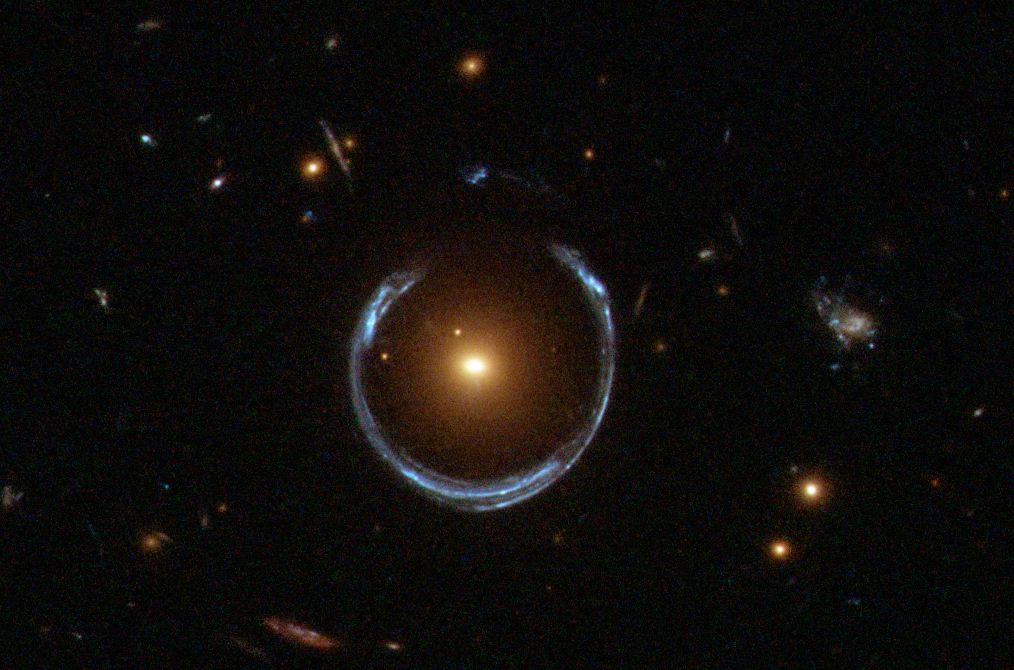
\includegraphics[trim={0cm, 2cm, 0cm, 0cm}, clip, height=4.5cm]{lensing_horseshoe}
 \end{subfigure}%
 \begin{subfigure}[t]{0.5\textwidth}
  \centering
  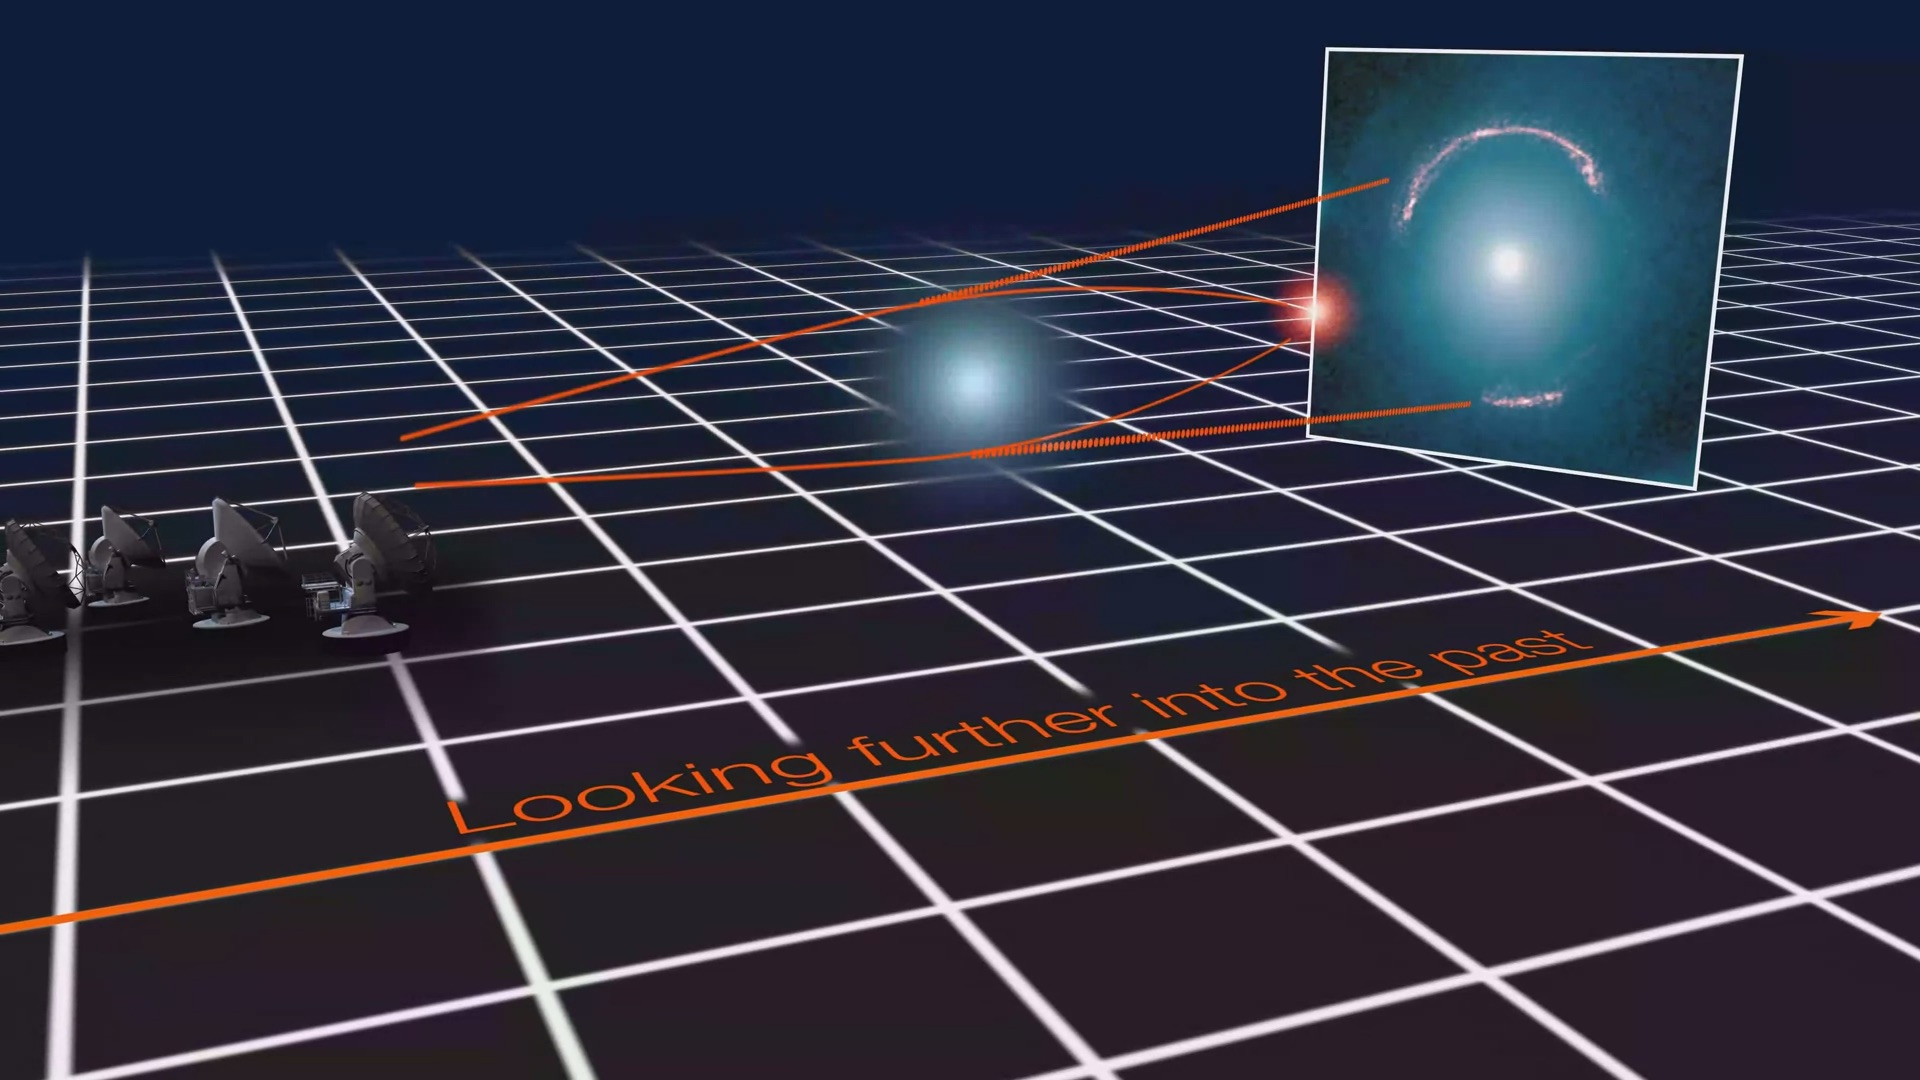
\includegraphics[trim={6cm, 0cm, 0cm, 0cm}, clip, height=4.5cm]{lensing_diagram}
 \end{subfigure}
 \caption{(left) an Einstein ``horseshoe" ring of a red galaxy distorting a blue galaxy behind it.  (right)
 A diagram of strong lensing.  The red source is bent by the blue lens, with the solid orange lines that connect
 to it representing the light's true trajectory.  The observer incorrectly views the source's
 position as indicated by the dashed orange lines, and the image behind them.  Image credit: (left) ESA/Hubble
 \& NASA (right) ALMA (NRAO/ESO/NAOJ)/Luis Calada (ESO)}
 \label{fig:lensing}
\end{figure}


In many astrophysical instances the lens' deflection of the source is much more subtle.  This is known as weak
lensing, and because of its minor effects is much more difficult to observe.  Astronomers must only consider a source's
shear because its luminosity is too low to be understood, and since the deviation in shear is small, systematic effects of
observing (i.e. atmosphere, instrument point spread function, noise, etc.) must be very small and well
understood \citeref{Paolis2016}.  Whereas strong lensing results from radiation passing around the lens, weak lensing
is the passage of light through a gravitational field where tidal effects distort the shape of the image.  Furthermore,
because galaxies are generally elliptical, deduction of the shear can be difficult to impossible.  Thus the gravitational
field is calculated statistically by randomly sampling galaxies from the known ellipticity distribution.  Since the
number of samples must equal the number of galaxies, this method is most effective when the number of galaxies is
large.

If the mass of the lens is well known, the luminous portion can be subtracted, yielding the fraction of DM.  This can typically
be done for strong lenses as shown in \figref{fig:lensing} but is more difficult for weak.

A galaxy collision provides a unique setting to study dark matter.  1E0657-56 (Bullet Cluster) is two galaxies that passed
through one another $\sim150$ million years ago at $4500_{-800}^{+1100}\ \mathrm{km\ s^{-1}}$ \citeref{Markevitch2004}.  \figref{fig:bullet_cluster} shows the x-ray map in pink and the mass
distribution from gravitational lensing in blue in the left panel, along with mass contours in the right.  The separation of
mass from baryonic matter can be explained by incorporating dark matter.  As the galaxies collide intergalactic dust interacts
and heats up, creating x-rays and slowing the speed at which they pass.  The dark matter does not interact and passes
through affected by only gravity.  In addition to providing evidence of dark matter, 1E0657-56 sets a limit on the
cross-section of dark matter self-interaction of $<1\ \mathrm{cm^{2}\ g^{-1}}$ \citeref{Markevitch2004}.  It also provides evidence
against modified gravity, an alternative hypothesis to dark matter, since the observed mass distributions should now lay
outside of the luminous content.



\begin{figure}[t!]
    \centering
    \begin{subfigure}[t]{0.45\textwidth}
        \centering
        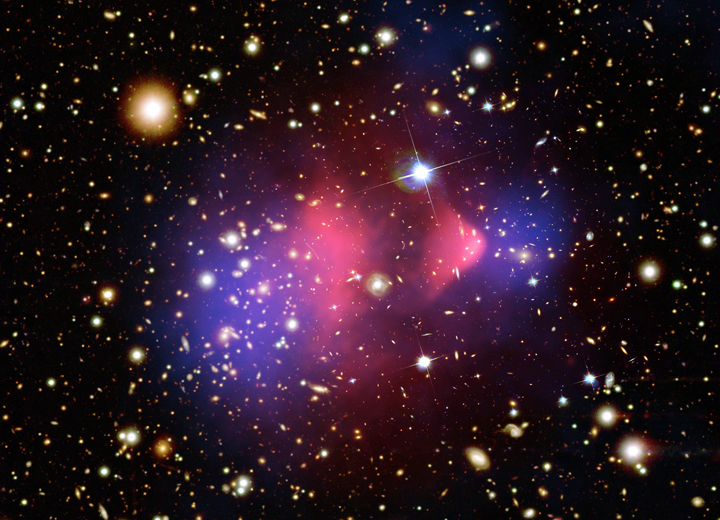
\includegraphics[height=4.5cm]{chandra_bullett_preview}
    \end{subfigure}%
    \begin{subfigure}[t]{0.45\textwidth}
        \centering
        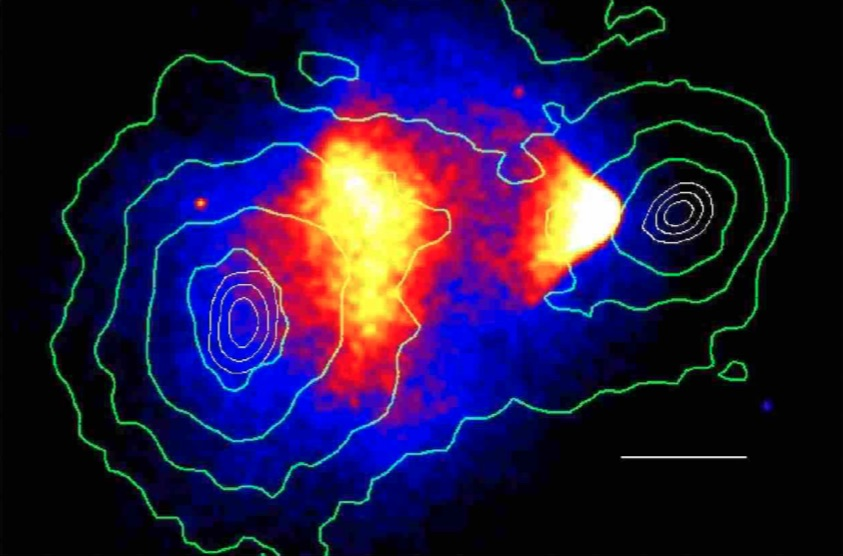
\includegraphics[height=4.5cm]{bullet_cluster_paper}
    \end{subfigure}
    \caption{X-ray emission from hot gas (pink) and mass centroids (blue) from gravitational lensing after cluster
	collision of 1E 0657-558.  The white bar in the right panel represents 200 kpc at cluster.  The separation
	between the colors provides evidence for Dark Matter.
	Image credit: (left) X-ray: NASA/CXC/CfA/M.Markevitch et al.; Optical: NASA/STScI; Magellan/U.Arizona/D.Clowe et al.;
	Lensing Map: NASA/STScI; ESO WFI; Magellan/U.Arizona/D.Clowe et al. (right) NASA, ESA, CXC, M. Brada\u{c}
	(University of California, Santa Barbara), and S. Allen (Stanford University)}
	\label{fig:bullet_cluster}
\end{figure}




%========
\subsection{Cosmic Microwave Background} \label{subsec:cmb}
The Cosmic Microwave Background (CMB) was accidentally discovered by Penzias and Wilson, for which they received
the Nobel Prize (\citeref{Penzias1965}).  It
is a remnant from shortly after the Big Bang ($\sim380,000\ \mathrm{yrs}$, $z\sim1100$, $T\sim3000\ \mr{K}$) and a near-perfect
blackbody at $2.725\ \mr{K}$ today (most precise measurement at $2.72548 \pm 0.00057\ \mr{K}$ \citeref{Fixsen2009}).  A CMB
photon is considered to have originated at the time of last scattering $t_{ls}$ and proceeded unperturbed since.

Deviations in the blackbody are small (root-mean square of $\delta T/T \sim 10^{-5}$) and the results of several
mechanisms at $t_{ls}$ that varied throughout space.  The dipole anisotropy results from
our motion with respect to the comoving rest frame of the CMB (\citeref{Smoot1991}).  Furthermore
energy density perturbations would cause fluctuations in gravitational potential $\delta \Phi$.  A
photon at larger $\delta \Phi$ at $t_{ls}$ would become blueshifted as its
potential decreases, while one at lower $\delta \Phi$ would be redshifted.  This effect is known as the
Sachs-Wolfe effect (\citeref{Sachs1967}).  Additional effects, including intrinsic fluctuations and acoustic
oscillations, are not discussed.

\begin{figure}
	\centering
	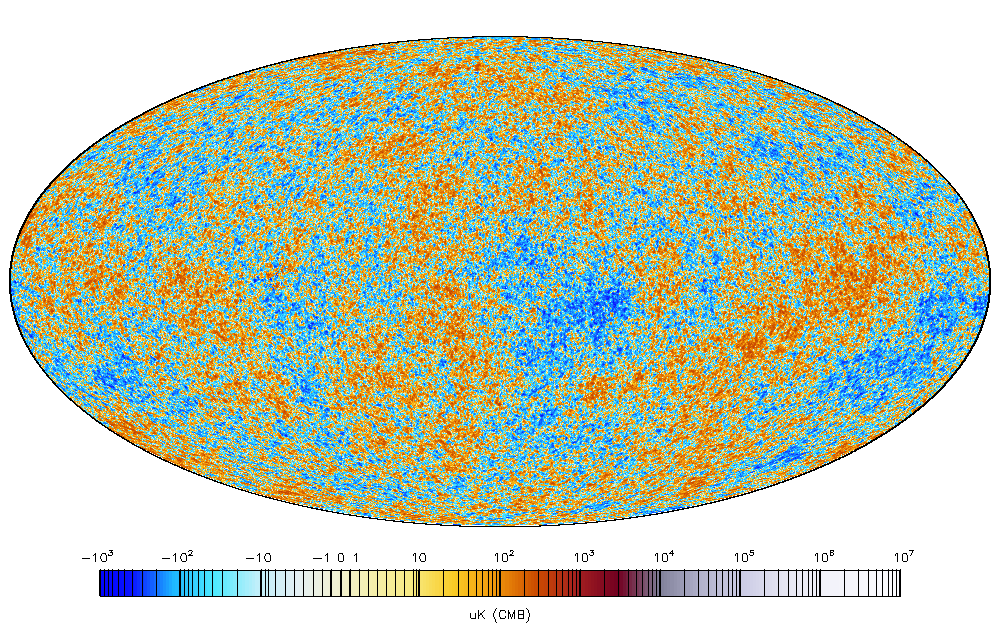
\includegraphics[width=0.8\textwidth]{PlanckFig_map_columbi1_IDL_HighDR_colbar_1000px_CMB_moll}
	\label{fig:planck_map}
\end{figure}


The CMB provides the most precise measurements on $\Omega_{b}$, $\Omega_{dm}$, $\Omega_{\Lambda}$, $\Omega_{r}$,
$H_{0}$, and many other cosmological parameters.  It has been precisely charted by several satellites since its
discovery, with the most recent being Planck (\citeref{Plack2011}).  The CMB is shown in \figref{fig:planck_map},
where fluctuations are on the order of $\sim 10^{\pm 3} \mu K$.  These fluctuations were caused by the number and
amount of each component - thus, by finding the correlation function

\begin{equation}
%C(\theta) = \Big \langle \frac{\delta T}{T}( \hat{n}) \frac{\delta T}{T} ( \hat{n}^\prime) \Big \rangle
C(\theta) = \Big \langle \delta T( \hat{n}) \delta T(\hat{n}^\prime) \Big \rangle
\end{equation}

\noindent we can identify the correction cosmological makeup.  To do this we make use of

\begin{equation}
\delta T = \sum\limits_{l=0}^{\infty} \sum\limits_{m=-l}^{l} a_{lm}Y_{lm}(\theta, \phi)
\end{equation}

\noindent where $\delta T = T(\theta, \phi) - \langle T \rangle$ for a given $\theta , \phi$
on the map, $Y_{lm}(\theta, \phi)$ corresponds to spherical harmonics, and $a_{lm}$ the preceding coefficients
with the condition that $\sum\limits_{l,m} |a_{lm}|^{2} = 1$.  This gives a correlation function of

\begin{equation}
C(\theta) = \frac{1}{4 \pi} \sum\limits_{l=0}^{\infty} (2l + 1) C_{l} P_{l}(cos \theta)
\end{equation}

\noindent where $P_{l}$ are the Legendre polynomials and $C_{l} = \frac{1}{2l + 1} \sum\limits_{m=-l}^{l} a_{lm}$.  The
only unknown is $C_{l}$, which is typically shown in an angular power spectrum with
$D_{l}^{TT} \equiv l(l+1)C_{l}/2\pi$ such as in \figref{fig:cmb_power_spectrum}.

\begin{figure}
%	\centering
	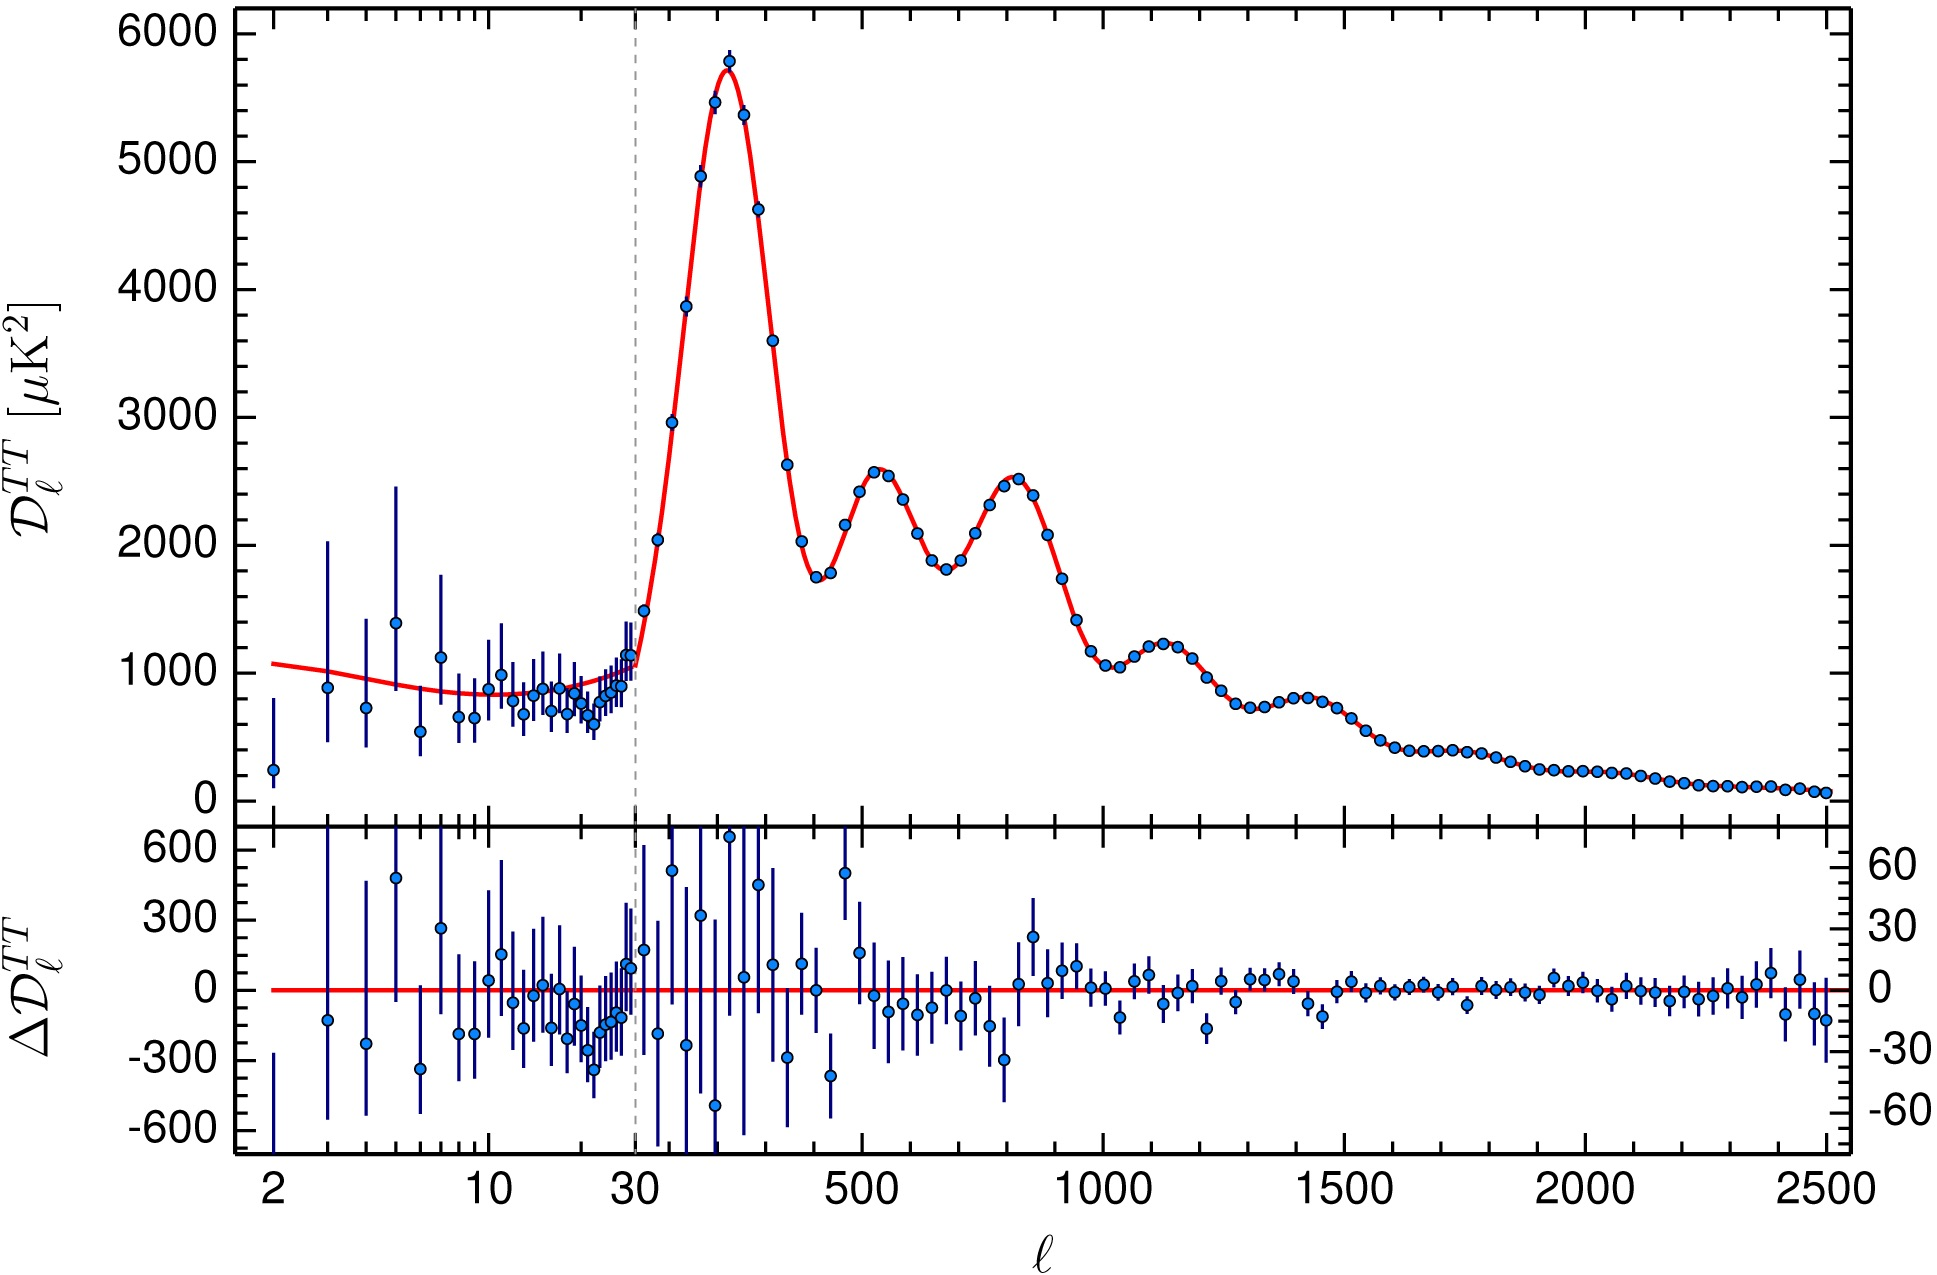
\includegraphics[width=0.8\textwidth]{cmb_power_spectrum}
	\centering
	\caption{Angular ower spectrum for CMB from Planck measurements, fit using the $\Lambda$CDM model.  Residuals
	are shown in bottom panel.  Image credit: \citeref{Planck2016}}
	\label{fig:cmb_power_spectrum}
\end{figure}

The first peak in the spectrum is related to the curvature of the universe, while the ratio of the heights of the
first and the second peaks provides details about the amount of baryonic matter.  The best fit gives
$H_{0} = 67.81 \pm 0.92\ \mathrm{km\ s^{-1}\ Mpc^{-1}}$, $\Omega_{\Lambda} = 0.692 \pm 0.012$,
$\Omega_{b} = 0.0484 \pm 0.0005$, $\Omega_{dm} = 0.258 \pm 0.004$, and
$\Omega_{k} \equiv 1 - \Omega_{\Lambda} - \Omega_{b} - \Omega_{dm} =  -0.005_{-0.017}^{+0.016}$.


%[5] Adams, F.C., Freese, K. & Guth, A.H. [1991], Phys. Rev. D43, 965.



%$\Omega_{m} = 0.308 \pm 0.012$
%$H_{0} = 67.81 \pm 0.92$
%$\Omega_{\Lambda} = 0.692 \pm 0.012$
%$\Omega_{b}h^{2} = 0.02226 \pm 0.00023$
%$\Omega_{c}h^{2} = 0.1186 \pm 0.0020$
%$N_{eff} = 3.046$
%$\Omega_{k} \equiv 1 - \Omega_{m} - \Omega_{\Lambda} = -0.005_{0.017}^{0.16}$ for $\Lambda CDM$

%========
%\subsection{Structure Formation} \label{subsec:structure}

%\endcsname

%====================================
\section[Dark Matter Candidates][Dark Matter Candidates]{Dark Matter Candidates}
\label{sec:dmcandidates}
Despite a strong claim for the existence of dark matter, there is no evidence for what its composition may
be.  A candidate for dark matter must have a lifetime much larger than the age of the universe, be electrically
neutral, and have a small matter-dark matter cross section.  Of course there may be more than one particle
that classifies as dark matter, but the sum of them should satisfy our observations of the universe.

%========
\subsection{Axions} \label{subsec:axions}
Axions were originally hypothesized by R.D. Peccei and Helen R. Quinn in 1977 as a solution to the strong CP
(charge and parity) problem (\citeref{Peccei1977}).  Quantum chromodynamics (QCD) predicts there should be
CP violation in strong interactions.

CP (charge and parity) violation in strong interactions has never been observed, despite its prediction
by quantum chromodynamics (QCD).  This forces a theoretically unjustified fine tuning of the model, which
is known as the strong CP problem.  Originally hypothesized by R.D. Peccei and Helen R. Quinn in 1977, the
axion - a new standard model particle - offered a solution (\citeref{Peccei1977}).  Shortly after it was
demonstrated that for axion decay constant $f_{a} > 10^{12}$ axions would be overproduced in the
early universe and cause the axion density $\Omega_{a} > 1 > \Omega_{dm}$ \citeref{Preskill1983}.  However,
a decay constant of $\sim 10^{12}$ could satisfy $\Omega_{dm}$.  Because the axion mass $m_{a}$ and $f_{a}$
are inversely proportional, one can then set a limit on $m_{a}$.
%The axion
%mass $m_{a} = 57(10^{11}GeV/f_{a})\ \mu$eV, which gives a lower bound of $m_{a} \sim 5\ \mu$eV.

Because axions naturally offer and explanation for dark matter there are a number of experiments dedicated to
finding them.  Cavity searches such as ADMX use a resonant microwave cavity inside a superconducting magnet
to convert axions in microwaves.  Others, like CASPEr apply NMR.


%========
\subsection{WIMPs} \label{subsec:wimps}
WIMPs (Weakly Interacting Massive Particles) are another favored candidate for dark matter.  As their name
suggests, they interact through the weak force and thereby would be difficult to observe.  They
are not constrained to the standard model, though would behave similarly
to neutrinos, which have a small cross-section and rarely interact with nuclei.  An additional requirement
is they must be produced early in the universe to account for observations of the CMB and galactic
structures.

At the beginning of the universe the temperature was hot enough where particles could annihilate with their
antiparticle counterpart and produce new particles, maintaining equilibrium.  As the universe cooled each
particle had a ``freeze-out", when they could no longer transfer freely to other particles.  Using the
$\Lambda$CDM model the density of DM in the universe today is given by

\begin{equation}
\Omega_{dm}h^{2} = \frac{3 \times 10^{-27}\ \mathrm{cm^{3}\ s^{-1}}}{\langle \sigma_{\mathrm{ann}} v \rangle}
\end{equation}

\noindent where $h$ is the Hubble Constant divided by 100 and $\langle \sigma_{\mathrm{ann}} v \rangle$ is
the thermally averaged self-annihilation cross section
for dark matter.  Assuming DM has a cross-section and mass on the order of the weak force, such a
particle would give roughly the correct relic density of DM.  This is known as the ``WIMP miracle".

Another appealing argument for WIMPs is super-symmetry (SUSY), which is theorized to solve some problems
with the standard model,
predict WIMP-like particles of similar masses.  This has historically been one of the favored arguments
for dark matter.

 %========
\subsection{Cold, Warm, or Hot} \label{subsec:hot_vs_cold}
An important property of dark is whether or not it was relativistic in the early universe.  Hot dark matter (HDM)
is defined as being relativistic at the time it decoupled from other components, $t_{mathrm{dec}}$, and at
matter-radiation equality, $t_{\mathrm{rm}}$.  Warm dark matter (WDM) would have been relativistic at $t_{\mathrm{dec}}$
but not at $t_{\mathrm{rm}}$.  Cold dark matter (CDM) would have been non-relativistic at both.  Candidates for CDM include
WIMPs, axions, and primordial black holes while WDM might be the gravitino.  Neutrinos are possible candidates for both
WDM and HDM.

Understanding which DM universe we live in can come from looking at structure in the universe.  Because the structure
today came from fluctuations in the earliest moments of the Big Bang (\secref{subsec:cmb}) the cosmological layout
can illuminate the answer.

In HDM the relativistic particles are able to smooth out density perturbations, which is known as free
streaming.  In this case the first structures to form would be superclusters, followed by smaller-scale
features.  Observations show that this is not the case; galaxies have been around since before the universe
was 1 billion years old ($z \sim 6$) and superclusters are just forming today (\citeref{Ryden2003}).

CDM allows the early density perturbations to persist, causing smaller structures to materialize first,
consistent with galaxy surveys between $\sim 1$ Mpc to the horizon.  At scales $< 1$ Mpc and
$M \sim 10^{11} \ M_{\odot}$ there are discrepancies, including under-dense cores for many galaxies that are DM-dominated
and significantly fewer satellite dwarf and small galaxies than predicted (\citeref{Moore1999}, \citeref{Klypin1999}).  Possible
solutions to the latter may be that dwarf galaxies have not accumulated enough baryonic matter to be visible
(\citeref{Simon2007}), merged, or been stripped by tidal forces of larger galaxies.

WDM has received a lot of interest since the CDM problems were observed.  Simulations have shown that
WDM would result in fewer subhalos, though other model-observation contradictions have been less
successful (\citeref{Bullock2017}, \citeref{Ogiya2017}).  However, since neutrinos have mass demonstrate there
was at least some non-CDM in the early universe.

Despite the problems with CDM, it remains the most favorable model for dark matter.  One possible outcome is
there is a mix of CDM and WDM, but if that's the case CDM would make up the considerable bulk of dark matter.


%====================================
\section[WIMP Detection Methods][WIMP Detection Methods]{WIMP Detection Methods}
\label{sec:detection}

 %========
\subsection{Colliders} \label{subsec:colliders}
One possible mechanism through which we might observe WIMP dark matter is through particle-antiparticle
annihilation.  This could be observed at particle colliders where energies can exceed
several TeV, thereby producing DM particle-antiparticle pairs, which
would escape undetected.  From momentum conservation there would be missing transverse energy (MET),
which would be carried in the DM.  The Large Hadron Collider (LHC) is investigating the quark sector with energies
exceeding 10 TeV, while the Large Electron-Positron (LEP) Collider is doing so for leptons at
$\sim 200$ GeV.  Both experiments are competitive at lower energies than noble gas experiments, particularly
for spin-dependent searches (\citeref{Fox2011}, \citeref{Alpigiani2017}).

Annihilation alone would not prove the discovery of dark matter, and would need
indirect or direct experiments to validate the results with their own detectors.  But
it would still be useful in narrowing the search region.


 %========
\subsection{Indirect Detection} \label{subsec:indirect}
Indirect detection looks for signatures of DM by observing standard model particles.  Such observables
may come from dark matter annihilation, wherein two DM particles annihilate and produce standard model
gamma rays or other particle-antiparticle pairs.  Alternatively if DM is unstable it may decay into
standard model particles that can be detected.

Indirect experiments look towards regions where they expect a large number of interactions.  The local
dark matter density is estimated to be 0.2-0.56 GeV/cm$^{3}$ (\citeref{Read2014}) and scientists are observing
the Sun, where they hope to find an observable flux of high energy neutrinos (\citeref{Ellis1988}).  Other theories suspect
DM annihilation in the galactic halo would produce
antiprotons, positrons, and gamma rays that would be detectable on Earth.  Because the the galactic center
has a large flux of cosmic rays it is difficult to distinguish dark matter from other astrophysical
sources.  Nearby ($\sim 50$ kpc) dwarf spherical
galaxies have become an attractive target where star formation regions have an expected low $\gamma$-ray
background (\citeref{Zitzer2016}).

Measurements of $\gamma$-rays would have to be from space because for the necessary energy range (GeV to TeV) photons interact
with matter via $e^{+}e^{-}$ pair production, so would not be able to pass through Earth's atmosphere.  However,
they can look for signatures such as showers of secondary particles and their Cerenkov
light as they pass through the atmosphere (\citeref{Bertone2005}).

% for Ellis1988 reference listed above get their references 6 and 7 and maybe 8 for citations, need access to PRL


 %========
\subsection{Direct Detection} \label{subsec:direct}
Direct detection looks for low energy ($\sim 1-100$ keV) nuclear recoil (a few theories predict DM-lepton
but they will not be discussed) (\citeref{Kopp2009}).  Given that the majority of dark matter must be
non-relativistic (\secref{subsec:hot_vs_cold}), we can calculate the differential recoil spectrum as \citeref{Undagoitia2016}

\begin{equation} \label{eq:dr_de}
\frac{dR}{dE}(E, t) = \frac{\rho_{0}}{m_{\chi}m_{\mathrm{A}}} \int_{v_{\mathrm{min}}}^{v_{\mathrm{esc}}}
v f(\boldsymbol{v}, t) \frac{d\sigma_{\chi}}{dE}(E, t)\ d^{3}v
\end{equation}

\noindent where $\rho_{0}$ is the local dark matter density of 0.2-0.56 GeV/cm$^{3}$ (\secref{subsec:indirect}), $m_{\chi}$ is
the mass of a
dark matter particle, $m_{\mathrm{A}}$ is the mass of the target element, $v_{\mathrm{esc}}$ is the escape velocity for WIMPs from the galaxy,
$f(\boldsymbol{v}, t)$ is the local velocity dispersion, and $\frac{d\sigma_{\chi}}{dE}(E, t)$ is the nucleon-DM differential
cross-section.  $v$ is the velocity of the DM in the rest frame of the detector.  The minimum velocity produce
a recoil of energy E is given by

\begin{equation}
v_{\mathrm{min}} = \sqrt{\frac{m_{\mathrm{A}} E}{2 \mu^{2}}}
\end{equation}

\noindent where the WIMP-nucleus reduced mass $\mu_{\mathrm{A}} = m_{\mathrm{A}} m_{\chi} /( m_{\mathrm{A}} + m_{\chi})$
and the velocity for
WIMPs to overcome the gravity of our galaxy has been measured to be $v_{\mathrm{esc}} = 533_{-41}^{+54}\ \mathrm{km\ s^{-1}}$
(\citeref{Piffl2014}).

Assuming the standard halo model (SHM)
Though there has been disagreement as to whether the DM velocity distribution can be described as Maxwell-Boltzmann
(\citeref{Diemand2004}, \citeref{Kuhlen2009}), we assume that this is the case.  For WIMP searches most experiments
are looking at spin-independent (SI) or spin-dependent (SD) interactions.  For spin-independent all nucleons
contribute equally.  For spin-dependent, atoms must have an odd number
of protons or neutrons since only unpaired nucleons contribute to the search.  The differential cross-section can then be written as

\begin{equation} \label{eq:diff_sigma_si}
\frac{d \sigma_{\chi}}{dE} = \frac{m_{\mathrm{A}}}{2 \mu_{\mathrm{A}}^{2} v^{2}} \big( \sigma_{0}^{\mathrm{SI}} F_{\mathrm{SI}}^{2}(E) +
\sigma_{0}^{\mathrm{SD}} F_{\mathrm{SD}}^{2}(E) \big)
\end{equation}

\noindent where $\sigma_{0}^{\mathrm{SI}}$ and $\sigma_{0}^{\mathrm{SD}}$ is the cross section at zero momentum for
spin-independent and spin-dependent DM.  $F_{\mathrm{SI}}^{2}(E)$ and $F_{\mathrm{SD}}^{2}(E)$ are the form factors, which
account for the cross-section decrease as energy increases (\citeref{Lewin1996}).  The SI form factor is
the Fourier transform of the mass density ground state, and for the parameterization given in \citeref{Helm1956} is given by

\begin{equation}
F_{\mathrm{SI}} = \frac{3 j_{1}(qr_{\mathrm{n}})}{qr_{\mathrm{n}}} e^{-(qs)^{2}/2}
\end{equation}

\noindent where $j_1(r_{\mathrm{n}}p)$ is a Bessel function of the first kind, $q = \sqrt{2m_{\mathrm{A}}E}$ is the momentum,
$r_{\mathrm{n}} = \sqrt{1.2A^{2/3} - 5s^{2}}$, and $s \sim 1$ fm is a measure of the nuclear skin (\citeref{Lewin1996},
\citeref{Engel1991}).  The cross section is then given by

\begin{equation} \label{eq:sigma_si}
\sigma_{0}^{\mathrm{SI}} = \sigma_{\mathrm{p}} \frac{\mu_{\mathrm{A}}^{2}}{\mu_{\mathrm{p}}^{2}} \frac{\big[ Z f^{p} +
(A - Z) f^{n} \big]^{2}}{(f^{p})^{2}}
\end{equation}

\noindent where $\sigma_{\mathrm{p}}$ is the cross section of a proton Z is the number of protons and $\mu_{\mathrm{p}}$ is
the WIMP-nucleon reduced mass. $f^{p/n}$ is the coupling strength for protons and neutrons, which are assumed to be
equivalent (see \citeref{Yaguna2017} for $f^{p} \neq f^{n}$).  Substituting \eqnref{eq:sigma_si} into \eqnref{eq:diff_sigma_si}
gives a spin-independent cross-section of

\begin{equation}
\frac{d \sigma_{\chi}}{dE} = \frac{m_{\mathrm{A}} \sigma_{\mathrm{p}}^{\mathrm{SI}}}{2 \mu_{\mathrm{p}}^{2} v^{2}}
 A^{2} \big| F(E) \big |^{2}
\end{equation}

\noindent This gives the differential rate as 

\begin{equation}
\label{eq:dr_de_final}
\frac{dR}{dE} = \frac{\rho_{0} A^{2} \sigma_{\mathrm{p}}^{\mathrm{SI}}}{2 m_{\mathrm{\chi}} \mu_{\mathrm{p}}^{2}}
  \big| F(E) \big |^{2} \int_{v_{\mathrm{min}}}^{v_{\mathrm{esc}}}
\frac{f(v)}{v}\ dv
\end{equation}

\noindent A direct detection experiment that is sensitive between energies $E_{\mathrm{min}}$ and $E_{\mathrm{max}}$ can count the number
of observed signals over a time $T$ for their target mass $M$ as

\begin{equation} \label{eq:counts}
N ( m_{\chi}, \sigma_{p}^{\mathrm{SI}}) = T \times M \times \int_{E_{\mathrm{min}}}^{E_{\mathrm{max}}} \frac{dR}{dE} dE
\end{equation}

\noindent \eqnref{eq:dr_de_final} and \eqref{eq:counts} state that the sensitivity of an experiment improves linearly with time and
target mass, but quadratically with $A$.  This makes heavier elements an important consideration when designing a direct detection
experiment.

%For SD interactions the cross-section is

%\begin{equation}
%\sigma_{0}^{\mathrm{SD}} = \frac{32}{\pi} \mu_{\mathrm{A}}^{2} G_{\mathrm{F}}^{2} \big[ a_{\mathrm{p}} \langle S^{\mathrm{p}} \rangle +
%a_{\mathrm{n}} \langle S^{\mathrm{n}} \rangle \big] \frac{J + 1}{J}
%\end{equation}

%\noindent where $G_{\mathrm{F}}$ is the Ferm coupling constant, $a_{\mathrm{p/n}}$ is the coupling constants, and $J$ is
%the total nuclear spin.




% https://journals.aps.org/rmp/abstract/10.1103/RevModPhys.28.214 for distribution of WIMP scatters assumed to be same
% as charge distribution derived from electron and muon scattering 


%correctly describes DM velocity
%as discussed in \secref{subsec:dynamics} assume the WIMP velocity the Maxwell-Boltzmann distribution



%Because current theory
%predicts the DM distribution to be in a halo around the galaxy (\secref{subsec:dynamics}), DM particles should
%be passing through Earth and - if they're WIMPS - interact with the nuclei of standard model atoms.



%The
%energy deposited in such a collision would be manifested as scintillation, excitation (nucleus or electron),
%ionization, or phonons.




%====================================
 \section[Direct Detection Experiments][Direct Detection Experiments]{Direct Detection Experiments}
 A moving particle that interacts with a detector will deposit some of its energy, causing different effects.  Some of the energy
 will be expelled as heat or propagated through the medium as phonons.  Additionally the atoms in the detector may become
 excited or ionized, producing scintillation and free electrons.  The different energy channels can be seen in
 \figref{fig:energy_channels}.  Experiments are probing all three of these observables, with many able to measure two
 simultaneously.
 
 Direct detection experiments look for some anomalous signal outside of their expected background.  This requires a comprehensive
 understanding of detector materials and physical location as both can produce radiation that will contaminate any signal.  For the
 former, major efforts are going into screening outsourced material and limiting the number of radioactive contaminates in
 production.  For on-site background radiation, shielding has been essential for many experiments who without would have orders
 of magnitude higher event rates.
 
 Even with a priori screening and effective shielding background events are inevitable.  Identifying a signal may be too
 difficult if the signal-to-background ratio is small.  In 1986 it was proposed
 that due to the Earth's relative motion around the Sun there should be a modulation in signal (\citeref{Drukier1986}).  Thus
 detectors could look for a an annual variation in event rate with a maximum in May, when the Earth's velocity around the
 Sun aligned with to the Sun's velocity around the galaxy.
 
 
 \begin{figure}
  \label{fig:energy_channels}
 \end{figure}
 
 
 %========
\subsection{Superheated Liquid Detectors} \label{subsubsec:bubbles}
Superheated liquid detectors have peak sensitivity to WIMP masses in the tens of GeV range.  Their limits for spin-independent
WIMPs are not as stringent as dual-phase noble gas detectors (\secref{subsec:dual_phase}), but they have consistently provided the
strongest constraints in the spin-dependent sector (\citeref{PICO2017}).  Their strong sensitivity comes from using fluorinated
halocarbons, as $^{19}$F is preferred over other detector materials due to its isotopic abundance of 100\% unpaired proton
almost always carrying 1/2 spin (\citeref{Ellis1991}, \citeref{PICASSO2012}).

At ambient temperatures and pressures fluorinated halocarbons in a metastable state.  A particle will transfer some of its heat,
which can result in nucleation and is observed acoustically or optically.  By varying the temperature and pressure settings
the superheated detectors can reduce $\gamma$ and $\beta$ interactions by a factor of 10$^{9}$, making them a great candidate for
SD dark matter discovery.

Additional superheated detector collaborations include PICASSO (\citeref{PICASSO2017}), COUPP (\citeref{COUPP2012}),
PICO (\citeref{PICO2017}), SIMPLE (\citeref{SIMPLE2012}), and MOSCAB (\citeref{MOSCAB2017}).


%When superheated liquid detectors were first considered for WIMP detectors there were some crucial points
%that needed to be addressed.  The downtime of such a detector was high because the temperature
%For WIMP searches modifications had to be made from the original
%devices including increased stability for near-continuous operation and operation as a counting experiment
%(\citeref{Pullia2014}).

 %========
\subsection{Scintillation Crystals} \label{subsec:crystals}
Another target for DM searches is highly radiopure scintillating crystals.  Typically sodium iodide (NaI) or cesium iodide (CsI) is chosen,
with NaI being the most common.  Their sensitivity to SI and SD, low energy threshold, can be run at room temperature,
and ability to run over long periods of time
make them an attractive option.  Doping with thallium causes an increase in wavelength providing high detection efficiency and large
crystal transparency (\citeref{Undagoitia2016}).  However, traces of $^{40}$K, and to a lesser extend $^{238}$U, $^{232}$Th,
and $^{87}$Rb in the NaI(Tl) crystals contribute a 3 \kevee peak (X-ray/Auger electron from $^{40}\mathrm{K} \rightarrow ^{40}\mathrm{Ar}$)
and flat background, which has made improved radiopurity an immediate goal (\citeref{Shields2015}).  Additionally, the scintillation
does not have unique features for different interactions, so particle discrimination is not possible, with the excepting of
multiple hits rejection.  Thus separating background from signal on and event by even basis is not possible.

The DAMA/NaI and its successor DAMA/LIBRA experiments are located underground at the Laboratori Nazionali del Gran Sassa (LNGS) in
Italy.  They use NaI(Tl) crystals that are sensitive.  For 14 annual cycles they have observed an annual modulation in the 2-6 \kevee
range with 9.3$\sigma$ (\citeref{DAMA2013}).  This would give WIMP masses of 10-15 GeV for scattering off Na
and 60-100 GeV for I.  Because NaI(Tl) cannot distinguish scatterings by different particles there is doubt on if their signal
is caused by WIMPs, or even dark matter.  Outside of spin-independent, spin-dependent or mixed coupling (\citeref{Bernabei2001})
and inelastic scattering (\citeref{Bernabei2002}) WIMPs 
have been considered.  Because DAMA/LIBRA cannot know if the interactions are with nuclei or electrons, alternative dark matter
electron-coupling models (\citeref{Bernabei2006}) have also been examined.  The results are controversial because other experiments
have surpassed the DAMA/LIBRA sensitivity and see no signal (\citeref{Aprile2017}).  This has provided motivation to explain the annual modulation via
standard particles.  Hypotheses include known variation in muon flux due to changing stratosphere temperatures, which exhibits
annual modulation in similar phase with DAMA/LIBRA's findings (\citeref{Blum2011}), an incomplete understanding of neutron backgrounds
(\citeref{Ralston2010}), or using a combination of muon-induced neutrons and soloar neutrinos (\citeref{2014Davis}) (though this
has been received pushback in \citeref{Barbea2014} and \citeref{Klinger2015}).


 %========
\subsection{Germanium Detectors} \label{subsec:germanium}
High purity germanium (HPGe) detectors measure ionization and offer great energy resolution.  As with scintillation crystals,
they can reach very low energies ($\sim$0.5 keV), making them a promising candidate for low-mass WIMPs ($\sim 10$ GeV).  It is not
possible to identify nuclear recoils from electronic, but p-type doped detectors have a dead layer on the surface and can use the
pulse rise time to reject background surface events.  In 2010 CoGeNT
announced it observed an annual modulation, similar to DAMA/LIBRA.  After continued observation showed a preference for the modulation
at 2.2$\sigma$ with a best-fit WIMP mass of $m_{\chi}\sim 8$ GeV (\citeref{CoGeNT2014}).  However, subsequent analyses with different
background assumptions showed that this preference is well below 1.7$\sigma$ (\citeref{Aalseth2014}, \citeref{Davis2014}).  Another
experiment, CDEX, uses the same setup as CoGeNT and found contradictory results (\citeref{CDEX2014}), as did CDMS II for NR only
(\citeref{CDMS2012}).


%========
\subsection{Cryogenic Bolometers} \label{subsec:bolometers}
Cryogenic bolometers are typically cooled to $10-100$ mK so they can detect phonons, allowing a low energy threshold and
outstanding energy resolution.  The CDMS collaboration uses silicon and germanium detectors where they measure both phonons
and ionization.  The ionization-to-phonon ratio is used for discrimination where less than 1 in $10^{6}$ of all ER events
are rejected in the $10-100$ keV range (\citeref{CDMS2015}).  In 2013 an excess of events was reported with a best-fit
WIMP mass of 8.6 GeV (\citeref{Agnese2013}).  However, later measurements did not observe such an excess, nor did EDELWEISS,
which has an analogous setup (\citeref{EDELWEISS2016}).

The CREST-II experiment measured phonons as well as scintillation in CaWO$_{4}$ crystals.  They also observed an excess of
events at WIMP masses of 11.6 at 4.2$\sigma$ and 25.3 GeV at 4.7$\sigma$ (\citeref{CRESST2012}), but in a later publication
ruled them out (\citeref{CRESST2015}).


 %========
\subsection{Liquid Noble Gas Detectors} \label{subsec:noble_gas}
Liquid noble gas detectors have led the field for spin-independent WIMP masses $\gtrsim 20$ GeV, as seen in
\figref{fig:si_sensitivity}.  Commissioned detectors have
used either liquid argon (LAr) or liquid xenon (LXe) and the DEAP/CLEAN collaboration is constructing a detector than can house
LAr and liquid neon (LNe) independently (\citeref{Kearns2012, CLEAN2015}).  Advantages of liquid noble gas detectors
include scaleability, particle discrimination, and self-shielding, among others.  As the target mass of these detectors passes
the 1-ton mark they are becoming sensitive to neutrinos, offering another branch of physics to study.

Liquid noble gas detectors can be single- or dual-phase.  Single-phase detectors measure only the scintillation and are generally
spherical and benefit from 4$\pi$ photo-detection.  Dual-phase apply an electric field to extract the free electrons for
measurement.  LXe experiments will be discussed in detail in \chapref{chap:liquid_xe}.


% read https://www.hindawi.com/journals/ahep/2014/387493/ to rewrite above section